\documentclass[12pt,notitle,letterpaper]{report}
% generated by Docutils <http://docutils.sourceforge.net/>
% rubber: set program xelatex
\usepackage{fontspec}
% \defaultfontfeatures{Scale=MatchLowercase}
% straight double quotes (defined T1 but missing in TU):
\ifdefined \UnicodeEncodingName
  \DeclareTextCommand{\textquotedbl}{\UnicodeEncodingName}{%
    {\addfontfeatures{RawFeature=-tlig,Mapping=}\char34}}%
\fi
\usepackage{ifthen}
\usepackage{alltt}
\usepackage{amsmath}
\usepackage{graphicx}

%%% Custom LaTeX preamble
% Linux Libertine (free, wide coverage, not only for Linux)
\setmainfont{Linux Libertine O}
\setsansfont{Linux Biolinum O}
\setmonofont[HyphenChar=None,Scale=MatchLowercase]{DejaVu Sans Mono}

%%% User specified packages and stylesheets
% embedded stylesheet: c:\Users\rodhh\Dropbox\projects\residence_remodel\rivtcalcs0001\docs\d00\pdf_style.sty
\makeatletter
%%
%% default LaTex report class style for rivtcalc 
%%
\usepackage{lastpage}
\usepackage{fancyhdr}
\usepackage{titlesec}
\usepackage{fontspec}
\usepackage{dejavu}
\usepackage{bm}
\usepackage{gensymb}
\usepackage[normalem]{ulem}
\usepackage{etoolbox}
\usepackage{tabulary}
\usepackage{geometry}
\usepackage{mathastext}
%% font size
\setmainfont{DejaVu Sans}[Scale=0.8]
\setsansfont{DejaVu Sans}[Scale=0.8]
\setmonofont{DejaVu Sans Mono}[Scale=0.8]
\setmathrm{Arial}
\setmathsf{Arial}
\setmathtt{Arial}
\DeclareMathSizes{10}
\renewcommand\familydefault\sfdefault
%% \usepackage[libertine]{newtxmath}

%% margins
\geometry{hmargin={0.5in,0.5in},vmargin={0.8in,0.8in}}
\setlength{\parindent}{0in}
\setlength{\parskip}{.1in}
\renewenvironment{quote}
  {\small\list{}{\rightmargin=0cm \leftmargin=0cm}%
   \item\relax}
  {\endlist}
%% pagestyle plain - table of contents
%% header
\pagestyle{fancy}
\fancyhf{}
\fancyhead[L]{\normalsize  Code Minimums - Carport Renovations}
\fancyhead[R]{\normalsize c0202 | \thepage}
\renewcommand\chaptermark[1]{\markboth{#1}{}} 
\renewcommand\sectionmark[1]{\markright{\thesection.\ #1}}
%% footer
\fancyfoot[C]{calc file: \jobname .py \hfill \today\ }
\renewcommand\headrulewidth{1pt}
\renewcommand\footrulewidth{1pt}
%% modify section headings - chapters
\titleformat{\chapter}
 [display]
 {\normalfont\large\bfseries}
 {}{0pt}
 {\large}
 [\vspace{2mm}\titlerule]
\titlespacing*{\chapter}{0pt}{-40pt}{12pt}
%% modify section headings - sections
\titleformat{\section}
 [display]
 {\normalfont\large\bfseries}
 {}{0pt}
 {\large}
 [\vspace{2mm}\titlerule]
\titlespacing*{\section}{0pt}{-40pt}{12pt}


\makeatother

%%% Fallback definitions for Docutils-specific commands
% hyperlinks:
\ifthenelse{\isundefined{\hypersetup}}{
  \usepackage[colorlinks=true,linkcolor=blue,urlcolor=blue]{hyperref}
  \usepackage{bookmark}
  \urlstyle{same} % normal text font (alternatives: tt, rm, sf)
}{}


%%% Body
\begin{document}
\setcounter{page}{21}


\vspace{.2in}   \textbf{Structural Deficiencies}   \hfill\textbf{SECTION 01}
\newline   \vspace{.05in}   {\color{black}\hrulefill}

The carport is a post and beam structure that was connected primarily by
gravity and friction and a few nails and screws with minimal capacity.

In addition there was significant post decay. Initially the posts were
supported on spread footings and the parking area was gravel. At some point
a few decades ago, the posts were encapsulated with a concrete slab up to 8
or 9 inches to provide a better parking surface. The encapsulating concrete
trapped water around the columns bases which caused serious decay and
eventually led to partial column failure, 90\% section loss in some cases
and differential settlement up to 7 inches.

\noindent{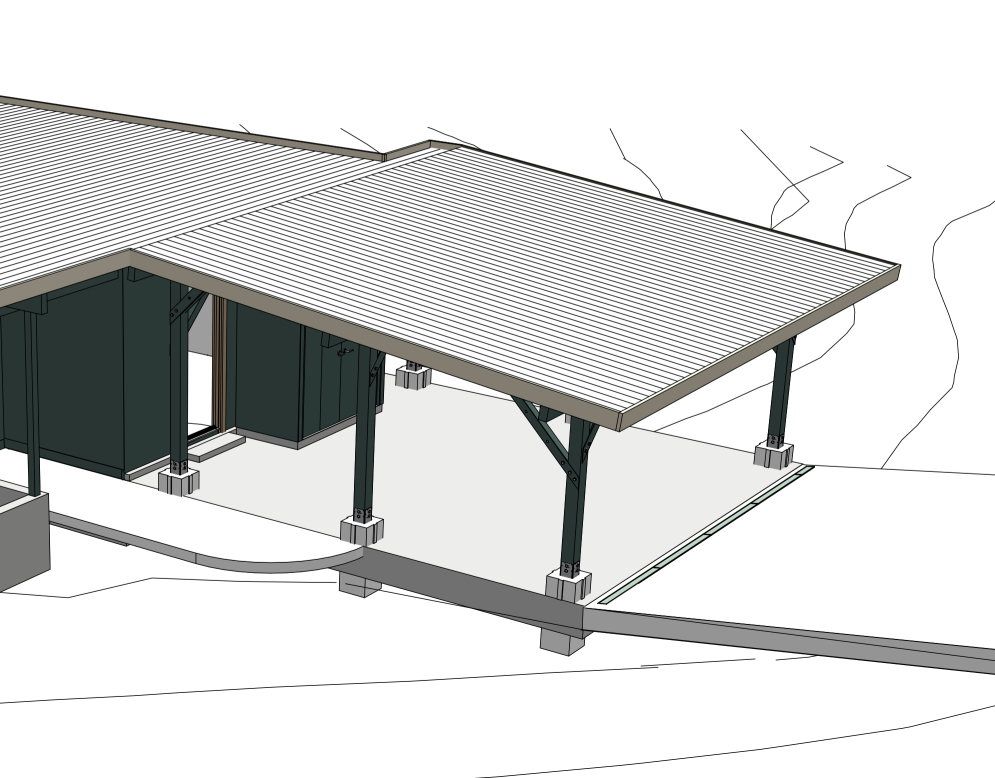
\includegraphics[width=0.900\linewidth]{C:/Users/rodhh/Dropbox/projects/residence_remodel/rivtcalcs0001/docs/d02_code_min/carport01.jpg}\hfill}

\textbf{Carport} \hfill {[} Fig: 0202.04 {]}

\vspace{.2in}   \textbf{Carport Repairs and Strengthening}   \hfill\textbf{SECTION 02}
\newline   \vspace{.05in}   {\color{black}\hrulefill}

Beam to beam, post to beam and brace to beam and post connections were
strengthened with 1/8\textquotedbl{} galvanized angles or plates that were attached with
lag bolts or galvanized threaded rods or bolts.

The carport was shored and leveled, the decayed bottom of the posts were
removed and new concrete foundations that raised the bottom of the posts
above the parking slab were installed to prevent further decay.  Each post
was postively anchored with double (orthogonal) bases.

\noindent{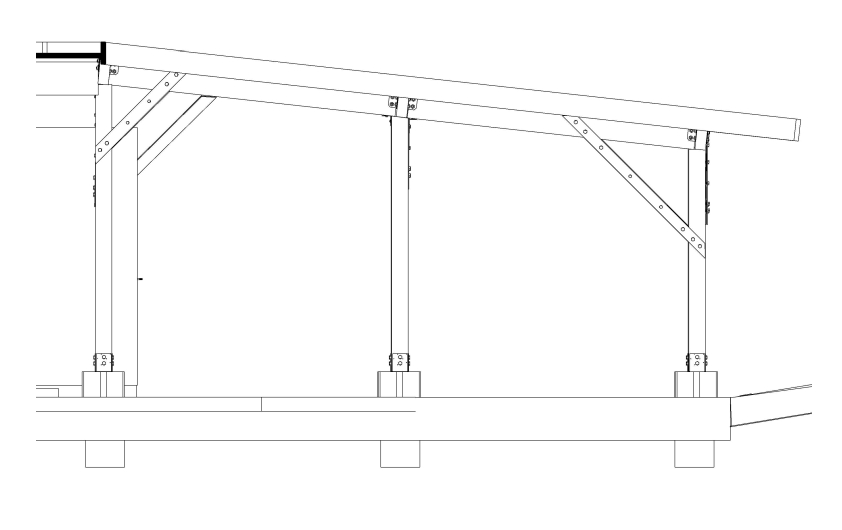
\includegraphics[width=0.800\linewidth]{C:/Users/rodhh/Dropbox/projects/residence_remodel/rivtcalcs0001/docs/d02_code_min/carport1.jpg}\hfill}

\textbf{Carport North Elevation} \hfill {[} Fig: 0202.05 {]}

\noindent{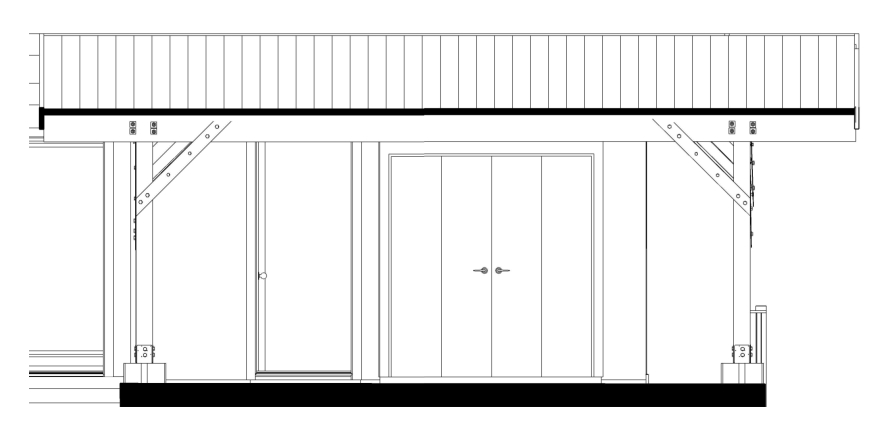
\includegraphics[width=0.800\linewidth]{C:/Users/rodhh/Dropbox/projects/residence_remodel/rivtcalcs0001/docs/d02_code_min/carport2.jpg}\hfill}

\textbf{Carport West Elevation} \hfill {[} Fig: 0202.06 {]}

\vspace{.2in}   \textbf{Seismic Model Inputs - CBC Requirements}   \hfill\textbf{SECTION 03}
\newline   \vspace{.05in}   {\color{black}\hrulefill}

Seismic demands on the carport were analyzed using a 3D FEM model (ETABS).
The model includes the geometry, loads and stiffness associated with the
post, beams and roof. Column bases, beam to post, and brace connections
were modeled as pins.

The in-plane stiffness of the T\&G roof is taken as 300 pounds/inch/inch
using test data from {[}USDA1972{]}.

{[}USDA1972{]} USDA Forest Products Laboratory. 1972. \textquotedbl{}Shear Stiffness Of Two-Inch
Wood Decks For Roof Systems\textquotedbl{}, U.S.D.A. Forest  Service RESEARCH  PAPER,
FPL 155 1972

\textbf{ASCE7-16; Risk II; Site D} \hfill  {[}Table: 0202.03{]}

\begin{tabulary}{1.0\textwidth}{LL}
%% {lr}
\hline
 Parameter   &    Value \\
\hline
 SS          &    1.512 \\
 S1          &    0.685 \\
 FA          &    1     \\
 FV          &    1.5   \\
 SMS         &    1.512 \\
 SM1         &    1.027 \\
 SDS         &    1.008 \\
 SD1         &    0.685 \\
 TL          &   12     \\
 PGA         &    0.603 \\
 PGAM        &    0.603 \\
 FPGA        &    1     \\
 LE          &    1     \\
\hline
%% 
\end{tabulary}
\vspace{.15in}

\textbf{Base shear coefficients} \hfill  {[}Table: 0202.04{]}

\begin{quote}
\begin{alltt}
==========  =======  =========  ===================
variable      value    [value]  description
==========  =======  =========  ===================
SDS            1.00       1.00  short period design
R1             3.25       3.25  reduction factor
omega          2.00       2.00  overstrength factor
==========  =======  =========  ===================
\end{alltt}
\end{quote}

\textbf{Seismic coefficent} \hfill {[} Equ: 0202.02{]}
%
\begin{equation*}
C_{s} = \frac{SDS}{R_{1}}
\end{equation*}
\begin{quote}
\begin{alltt}
====================  ========  =====
        C_s              R1      SDS
====================  ========  =====
0.31 [-]  [0.31 [-]]  3.25 [-]   [-]
====================  ========  =====
\end{alltt}
\end{quote}

\end{document}
